% TikZ body (shared by main.tex and the standalone wrapper).
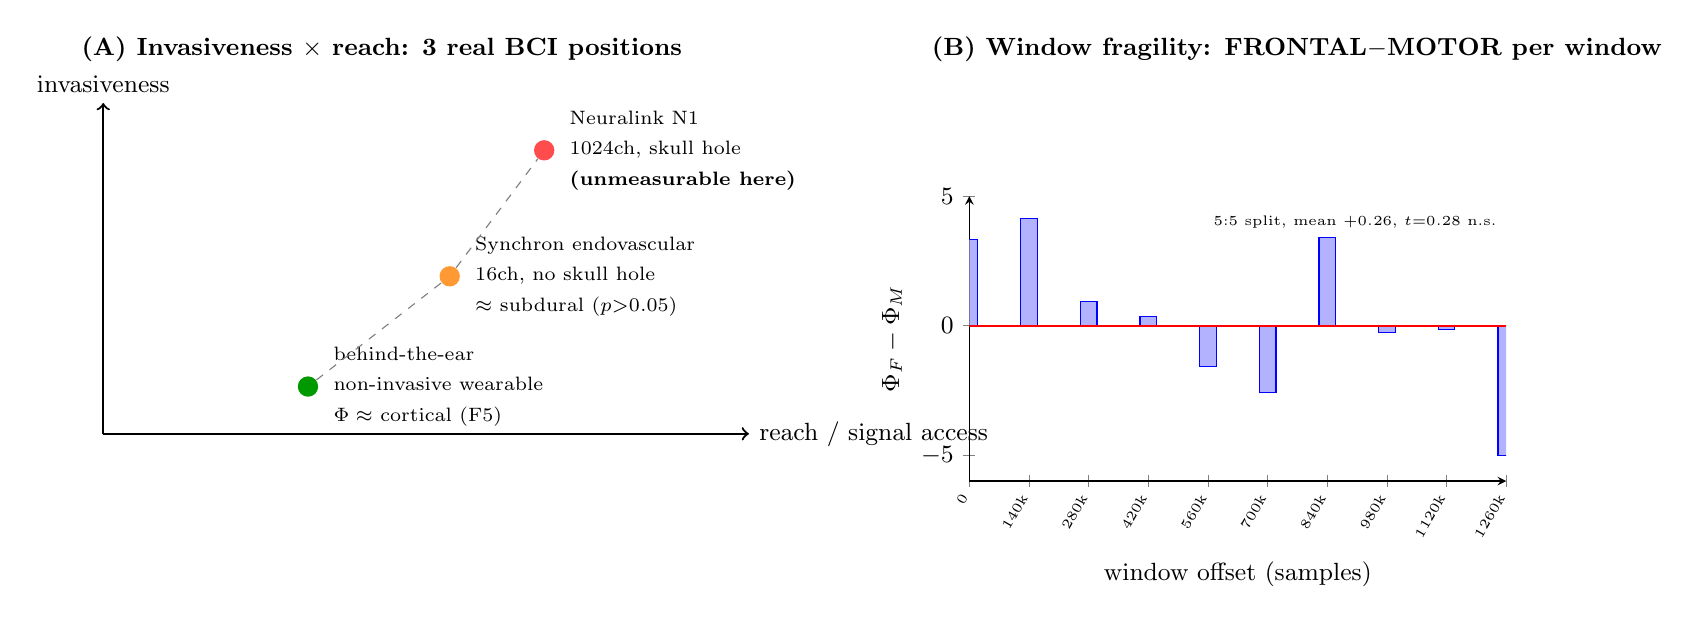
\begin{tikzpicture}[font=\small]

% ===== Panel A: invasiveness x reach 3-position ladder =====
\begin{scope}
  \node[anchor=south west] at (-0.4,4.6) {\textbf{(A) Invasiveness $\times$ reach: 3 real BCI positions}};
  \draw[->,thick] (0,0) -- (8.2,0) node[right] {reach / signal access};
  \draw[->,thick] (0,0) -- (0,4.2) node[above] {invasiveness};

  \node[circle,fill=red!70,inner sep=2.6pt] (n1) at (5.6,3.6) {};
  \node[circle,fill=orange!80,inner sep=2.6pt] (syn) at (4.4,2.0) {};
  \node[circle,fill=green!60!black,inner sep=2.6pt] (ear) at (2.6,0.6) {};

  \node[align=left,anchor=west] at (5.8,3.6) {\scriptsize Neuralink N1\\ \scriptsize 1024ch, skull hole\\ \scriptsize \textbf{(unmeasurable here)}};
  \node[align=left,anchor=west] at (4.6,2.0) {\scriptsize Synchron endovascular\\ \scriptsize 16ch, no skull hole\\ \scriptsize $\approx$ subdural ($p{>}0.05$)};
  \node[align=left,anchor=west] at (2.8,0.6) {\scriptsize behind-the-ear\\ \scriptsize non-invasive wearable\\ \scriptsize $\Phi\approx$ cortical (F5)};

  \draw[dashed,gray] (ear) -- (syn) -- (n1);
\end{scope}

% ===== Panel B: window-fragility 5:5 split =====
\begin{scope}[xshift=11cm]
  \node[anchor=south west] at (-0.6,4.6) {\textbf{(B) Window fragility: FRONTAL$-$MOTOR per window}};
  \begin{axis}[
      at={(0,-0.6cm)},
      width=8.4cm, height=5.2cm,
      ybar, bar width=6pt,
      ymin=-6, ymax=5,
      xtick=data,
      xticklabel style={rotate=60,anchor=east,font=\tiny},
      symbolic x coords={0,140k,280k,420k,560k,700k,840k,980k,1120k,1260k},
      ylabel={$\Phi_{F}-\Phi_{M}$},
      xlabel={window offset (samples)},
      axis lines=left,
      every axis plot/.append style={fill=blue!55},
    ]
    \addplot coordinates {
      (0,3.326) (140k,4.141) (280k,0.924) (420k,0.366) (560k,-1.579)
      (700k,-2.583) (840k,3.400) (980k,-0.275) (1120k,-0.147) (1260k,-5.020) };
    \draw[red,thick] (axis cs:0,0) -- (axis cs:1260k,0);
    \node[anchor=north east,font=\tiny] at (axis cs:1260k,4.6)
      {5:5 split,\ mean $+0.26$,\ $t{=}0.28$\ n.s.};
  \end{axis}
\end{scope}

\end{tikzpicture}
